\documentclass[11pt, a4paper, twoside, openright]{report}
\usepackage{float} % lets you have non-floating floats
\usepackage{tabularx}
\usepackage{booktabs}
\usepackage{graphicx}
\usepackage{caption}
\usepackage{url} % for typesetting urls
%  We don't want figures to float so we define
\newfloat{fig}{thp}{lof}[chapter]
\floatname{fig}{Figure}


\title{Genetic Programming for Antarctic Ice Sheet Modelling}
\author{Samuel Mata}
\usepackage[font, ecs]{vuwproject} 
\supervisors{Dr. Bach Nguyen, Dr. Bing Xue}
\otherdegree{Bachelor of Science with Honors in Artificial Intelligence}
\date{}
\begin{document}
\frontmatter

%%%%%%%%%%%%%%%%%%%%%%%%%%%%%%%%%%%%%%%%%%%%%%%%%%%%%%%

\begin{abstract}
  This project aims to investigate and evaluate the use of Genetic
  Programming \textit{(GP)} and Evolutionary Learning techniques for
  the long-term modelling of Antarctic Ice Sheet measurements. 
\end{abstract}

%%%%%%%%%%%%%%%%%%%%%%%%%%%%%%%%%%%%%%%%%%%%%%%%%%%%%%%

\maketitle

\tableofcontents

%%%%%%%%%%%%%%%%%%%%%%%%%%%%%%%%%%%%%%%%%%%%%%%%%%%%%%%

\mainmatter

%%%%%%%%%%%%%%%%%%%%%%%%%%%%%%%%%%%%%%%%%%%%%%%%%%%%%%%

\chapter*{1. Introduction}
\section*{1.1 Problem Statement}
\section*{1.2 Project Objectives}

%%%%%%%%%%%%%%%%%%%%%%%%%%%%%%%%%%%%%%%%%%%%%%%%%%%%%%%

\chapter*{2. Background}
- Do not focus on this for progress report
- Machine learning
- Read extra papers if have time
- classification / regression
- How technology relates to problem

\section*{2.1 Antarctic Ice Sheet Modelling}

\section*{2.2 Machine Learning}


%%%%%%%%%%%%%%%%%%%%%%%%%%%%%%%%%%%%%%%%%%%%%%%%%%%%%%%

\chapter*{3. Exploratory Data Analysis}
- Show understanding of dataset
- Show original data
- Show difference between original data and processed dataset
- What findings have been found

\section*{3.1 Description of Initial Dataset}

The dataset used in this project was obtained from Victoria University's Antarctic Research Center.
It details the results of several physics-based simulations in effort to predict the future state of the Antarctic Ice Sheet.
Specifically, the dataset consistutes 86 files, each representing 1 year of simulation data \textit{(Ranging from 2015 to 2100 inclusive)}.
Each of these files contains 2601 datapoints \textit{(Totalling 223,686 across all files)}, with each datapoint representing one cell in 
a 51x51 grid of the Antarctic Ice Sheet. 8 measures are counted for each datapoint, which can be described in three forms:
\begin{description}
  \item[Positional Constants] These encode the constant positional data of each cell in a pair of 
  \texttt{x\_coordinate} and \texttt{y\_coordinate} values.
  Both of these values range from -3,040,000 to 3,040,000 in discrete intervals of 121,600,
  with the grid being centered around point \textit{(0,0)}, which lies on the South Pole.
  These are not directly useful for modelling without feature engineering, and primarily serve as a reference for the grid.
  \item[Input Forcings] These are the primary inputs to be utilized in model prediction.
  These include 3 continuous features; \texttt{precipitation}, \texttt{air\_temperature}, and \texttt{ocean\_temperature}, 
  which are the respective measurements for each cell provided by the physical simulation. 
  \item[Outputs] These are the target outputs for the model to predict. 
  These include 2 continuous measurements; \texttt{ice\_thickness} and \texttt{ice\_velocity},
  which represent the respective thickness and velocity of the ice in each cell. 
  This also includes \texttt{ice\_mask}, which is a discrete value representing
  whether a cell contains grounded ice, floating ice, or no ice at all \textit{(i.e. open ocean)}.
\end{description}

\section*{3.2 Initial Data Cleaning}
Initial analysis was performed without preprocessing to understand the nature of the initial dataset.
This analysis excludes the positional constants \texttt{x\_coordinate} and \texttt{y\_coordinate},
as these are used for reference and not for prediction or evaluation.

Some minor data cleaning was performed before analysis, so as not to skew the results.
Most prominently, several values in the dataset were found to be filler values original
NaN \textit{(Not a Number - used to represent empty or faulty data points)}.

\begin{table}[h!]
  \centering
  \begin{tabular}{|l|r|r|}
  \hline
  Measure & Count & Proportion of Measure \\ \hline
  ice\_thickness & 143,819 & 64.29\% \\ \hline
  ice\_velocity & 146,083 & 65.30\% \\ \hline
  ice\_mask & 124 & \textless{0.01}\% \\ \hline
  ocean\_temperature & 29,584 & 13.22\% \\ \hline
  precipitation & 385 & \textless{0.01}\% \\ \hline
  \end{tabular}
  \caption{Counts of NaN and Filler Values in Dataset}
  \label{table:measure_counts}
\end{table}
  
The large proportion of NaN and filler values in the dataset is due to the relationship between ocean and ice cells.
The majority of cells are in the ocean surrounding the ice sheet - and thus do not have ice measurements. This
causes the ice measurements \textit{(ice\_thickness, ice\_velocity, ice\_mask)} to be NaN or filler values in these cells
\textit{(typically 0)}. Inversely, the ocean temperature measurements are NaN or filler values in cells containing ice
\textit{(typically 9.969...e+36)}, though this value is also used for cells without any measurement taken.

For ocean temperature values, the datapoints containing NaN or filler values were removed from the dataset.
This was done as these values are exclusively around the perimeter of the collected data, and only used to 
provide a square grid despite the circular nature of the collected data. This can be viewed with a spatial
heatmap of the ocean temperature values, which shows a clear circular border around the data where these
values are not present.

\begin{figure}[ht]
  \centering
  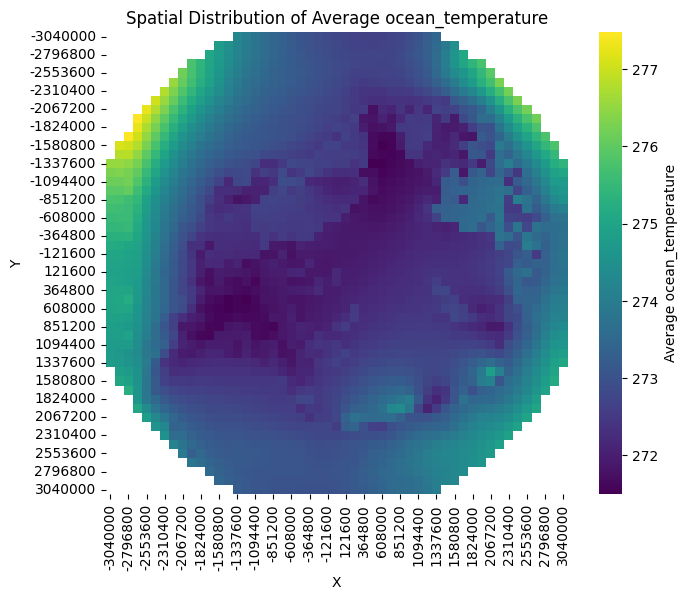
\includegraphics[width=0.75\textwidth]{images/ocean_temperature_spatial_heatmap.png}
  \caption{Spatial Heatmap of Average Ocean Temperatue Values}
  \label{fig:example-image}
\end{figure}

Filler values for ice mask were set to 4, as this value is used to represent open ocean.
Additionally, all measures were quantised into integers to reflect the discrete nature of
the variable, and to discard some minor variations in values. Ice velocity and ice thickness
do not have set values for ocean cells, so these were left as NaN values for the initial analysis.

Finally, the few NaN values in the precipitation variable were filled with the mean of the variable, as these
appeared randomly distributed throughout the dataset.

\section*{3.3 Univariate Analysis}
With initial data cleaning complete, univariate analysis can be completed on each variable. This was first done with 

\begin{table}
  \centering
  \caption{Summary Statistics for Input Forcings}
  \begin{tabular}{lcccccccc}
      \toprule
      & \textbf{Count} & \textbf{Mean} & \textbf{Std} & \textbf{Min} & \textbf{25\%} & \textbf{50\%} & \textbf{75\%} & \textbf{Max} \\
      \midrule
      \textbf{Precipitation} & 223686 & 575.61 & 364.76 & -522.47 & 204.15 & 638.85 & 871.18 & 2459.46 \\
      \textbf{Air Temperature} & 223686 & 258.14 & 16.93 & 214.14 & 245.16 & 265.52 & 271.24 & 297.43 \\
      \textbf{Ocean Temperature} & 194102 & 273.12 & 1.09 & 271.19 & 272.31 & 272.89 & 273.69 & 277.98 \\
      \bottomrule
  \end{tabular}
\end{table}

\begin{figure}
  \centering
  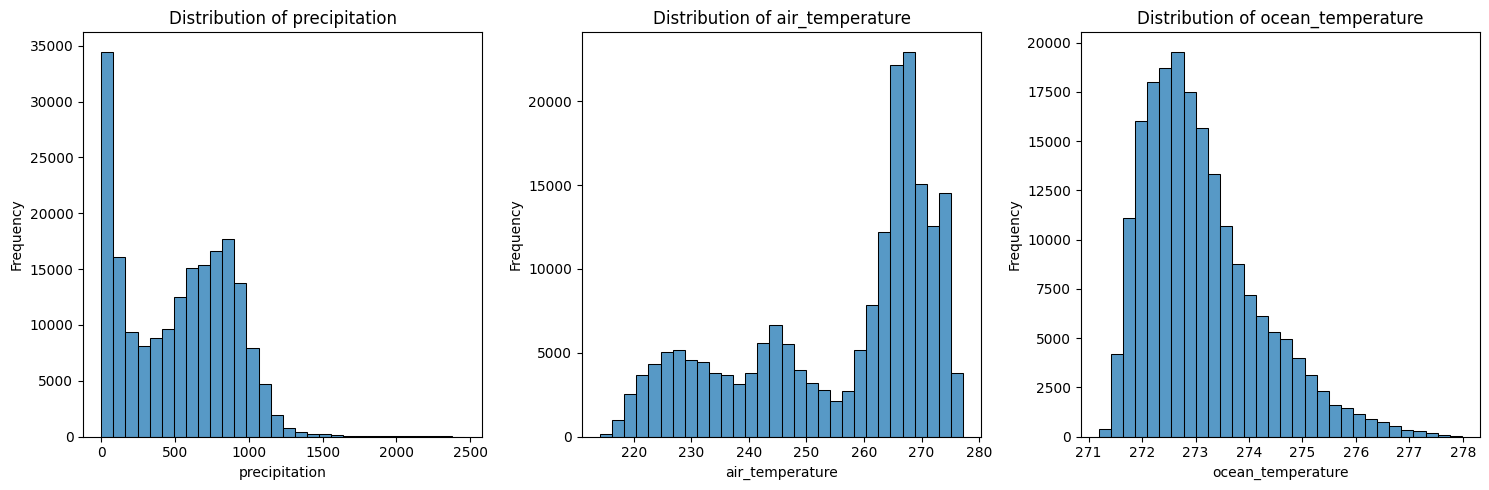
\includegraphics[width=1.04\textwidth]{images/input_forcing_distributions.png}
  \caption{Distribution of Input Forcings in Dataset}
  \label{fig:example-image}
\end{figure}

ANALYSIS

\begin{table}
  \centering
  \caption{Summary Statistics for Target Outputs}
  \begin{tabular}{lcccccccc}
      \toprule
      & \textbf{Count} & \textbf{Mean} & \textbf{Std} & \textbf{Min} & \textbf{25\%} & \textbf{50\%} & \textbf{75\%} & \textbf{Max} \\
      \midrule
      \textbf{Ice Thickness} & 79867 & 1901.61 & 1084.26 & 0.00 & 922.46 & 2061.50 & 2823.69 & 4614.76 \\
      \textbf{Ice Velocity}  & 77603 & 86.49 & 298.34 & 0.00 & 2.78 & 8.63 & 29.53 & 12527.31 \\
      \textbf{Ice Mask}      & 223562 & 3.33 & 0.93 & 0.51 & 2.00 & 4.00 & 4.00 & 4.36 \\
      \bottomrule
  \end{tabular}
\end{table}

\begin{figure}
  \centering
  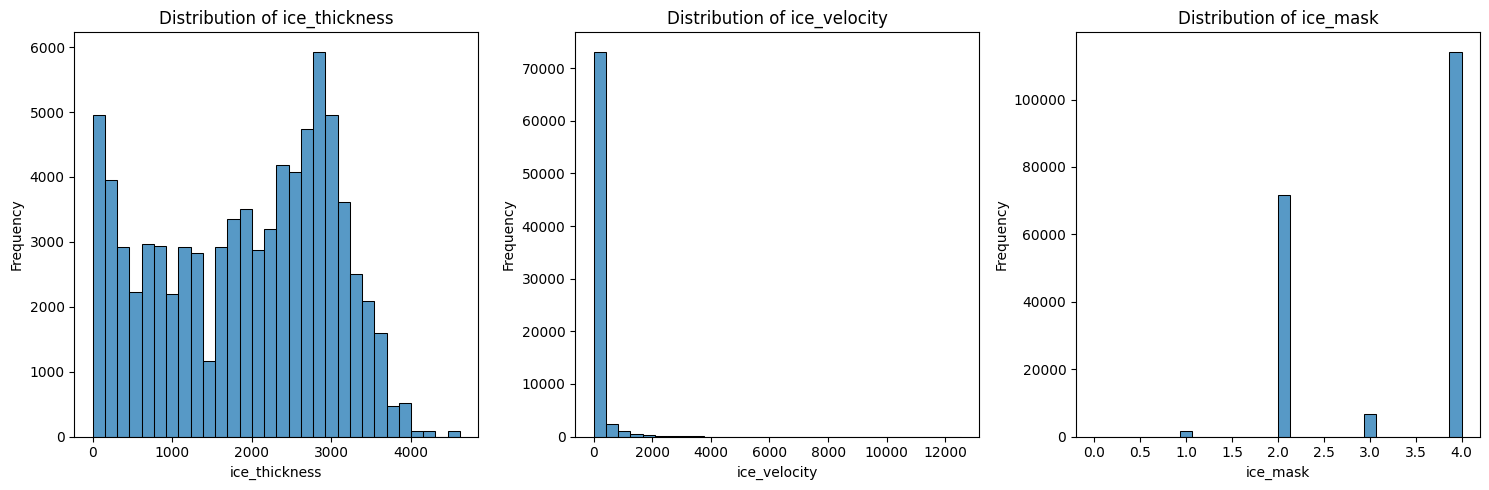
\includegraphics[width=1.02\textwidth]{images/target_output_distributions.png}
  \caption{Distribution of Target Outputs in Dataset}
  \label{fig:example-image}
\end{figure}

ANALYSIS

\section*{3.4 Spatial Analysis}

\section*{3.5 Temporal Analysis}

\section*{3.6 Correlation Analysis}

\section*{3.7 Preprocessing}

Several stages of preprocessing were performed on the dataset as directed by the analysis.
This included several

- Talk about feature before -> why a change is justified -> after

\begin{description}
  \item[] 
\end{description}

\subsection*{3.8 Feature Engineering}


%%%%%%%%%%%%%%%%%%%%%%%%%%%%%%%%%%%%%%%%%%%%%%%%%%%%%%%

\section*{4. Conclusions}
- What I have learnt from this
- Identify problems in solution
- what are potential future works


%%%%%%%%%%%%%%%%%%%%%%%%%%%%%%%%%%%%%%%%%%%%%%%%%%%%%%%
\backmatter
%%%%%%%%%%%%%%%%%%%%%%%%%%%%%%%%%%%%%%%%%%%%%%%%%%%%%%%

%\bibliographystyle{ieeetr}
\bibliographystyle{acm}
\bibliography{sample}
\end{document}
